% Chapter 4 from the standard thesis template
% that contains an adv. example table and figure.
\chapter{SOFTWARE DEFINED RADIOMETER IMPLEMENTATION}\label{ch:implementation}

This chapter examines the implementation of a software defined radio based radiometer.  First we will examine requirements of both a traditional radiometer and a digital radiometer.  Next we will map the traditional radiometer components discussed in chapter \ref{ch:background} to their digital counterparts.  Finally a high level overview of a software defined radio based radiometer will be given.

\section{Requirements}\label{requirements}

This section discusses the hardware and software requirements used to drive the selection of the hardware and software platforms use to implement our software defined radio based radiometer.  

\emph{Hardware Requirements.}  The capabilities of existing traditional radiometers were the primary driving force in setting the requirements of our hardware development platform.  Dr. Brian Hornbuckle from the Electrical and Computer Engineering and Agronomy department at Iowa State University was consulted with respect to key specifications of his radiometer.  Additionally, the specifications of other radiometers were examined. 

Table \ref{rad_performance} summarizes the specification of three parameters that were decided upon for selecting our hardware development platform, based on our investigation.  This lead to the selection of the N200 software defined radio platform with a DBSRX2 daughter board from Ettus Research as our platform.  Section \ref{SDR_platform} provides more in depth information on the hardware used and why it was selected.

\begin{table}[h!tb] \centering
\isucaption{Required Radiometer performance}
\label{rad_performance}
% Use: \begin{tabular{|lcc|} to put table in a box
\begin{tabular}{lcc} \hline
\textbf{Parameter} & \textbf{Value} & \textbf{Units} \\ \hline
Minimum bandwidth & 20 & MHz \\
Operational frequency & 1400 - 1420 & MHz \\
$NE\Delta T$ (sensitivity) & 1 & Kelvin \\ \hline
\end{tabular}
\end{table}

\emph{Software Requirements.}  Since an objective of this work was to help make radiometers more wildly accessible to the general research and education communities, a requirement of the development software was ease of use.  Additionally, the user interfaces developed with these software tools needed to be easy to use, while providing sufficient computing efficiency for the signal processing required for radiometry.

GNURadio met the stated requirements.  It includes a supplemental software package called GNURadio Companion (GRC), which uses a graphical interface for creating a radio environment.  GNURadio and GRC are discussed in greater detail in Section \ref{software_platform}.

%Since an easy to use system was a requirement in the selection of the software.  GNURadio was selected as it includes GNURadio Companion (GRC), a supplemental program which uses a graphical interface for creating the radio environment.  GNURadio and GRC is discussed in greater detail in Chapter \ref{ch:background}, section \ref{software_platform}. 

\section{Mapping Traditional Radiometer Functions to a Software Defined Radio Based Radiometer}

The use of a software defined radio (SDR) to implement a radiometer requires mapping components of a traditional radiometer to SDR-based technology.  This section presents the mapping of three such components for implementing our SDR-based radiometer.  These components are:  1) power measurement, 2) integration, and 3) filtering.

\subsection{Power measurement}

A traditional radiometer uses a device called a square law detector to measure power.  It transforms an input signal into an output voltage whose square is proportional to the input signal power.  Figure \ref{square_law_simple} shows a simple circuit diagram.  Mathematically it takes an input signal (x) and gives an output (y) as the square of the input as shown in equation \ref{square_eq}.

\begin{equation}\label{square_eq}
y = x^2
\end{equation}

%The random noise we measure is noise that is generated due to thermal agitation in the median.  This random noise has peak values but the mean value of the noise is zero.  The square-law detector takes the peak values of this random noise and this results in the total power detected.

{\begin{figure}[h!tb] 
\centering
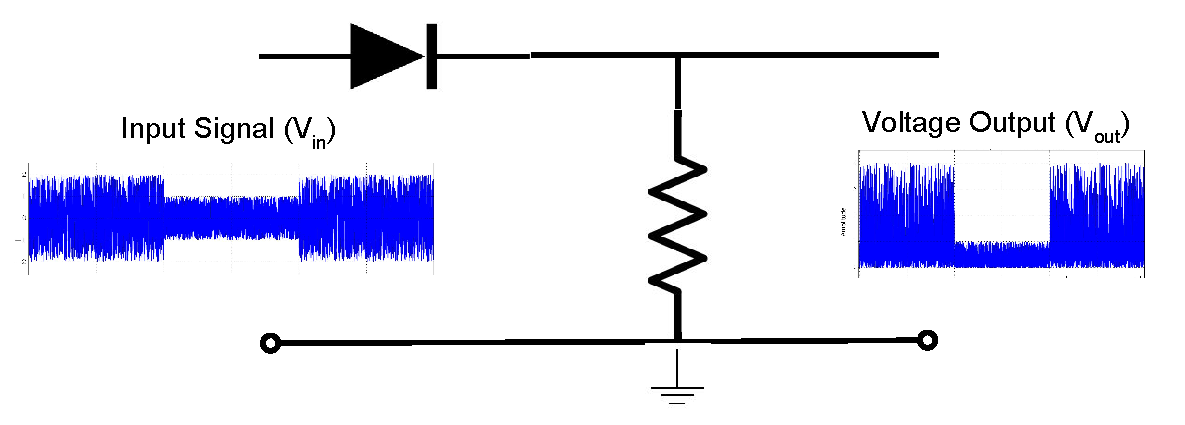
\includegraphics[width=17cm]{Images/square_law.pdf}
\isucaption{A simple diagram of a square-law detector.}
\label{square_law_simple}
\end{figure}
}

The software defined radio based radiometer operates in the same manor as a traditional radiometer.  The input signal, represented as I (in-phase) and Q (quadrature-phase), is squared and summed to produce an output ($P_{out}$).  Equation \ref{sdr_x2} gives the mathematical representation of a software defined radio based radiometer implementation of a square law detector[\cite{Rashid}]. 

\begin{equation}\label{sdr_x2}
I^2+Q^2 = P_{out}
\end{equation}

Figure \ref{square_block} shows the block within GNURadio Companion that performs the function of total power measurement.  In Figure \ref{square_block}, the block labeled as A performs mathematically the power detection as shown in Equation \ref{sdr_x2}.  Block C decimates the data to reduce the sample size and thus reduce the file size of the data.  

{\begin{figure}[h!tb] 
\centering
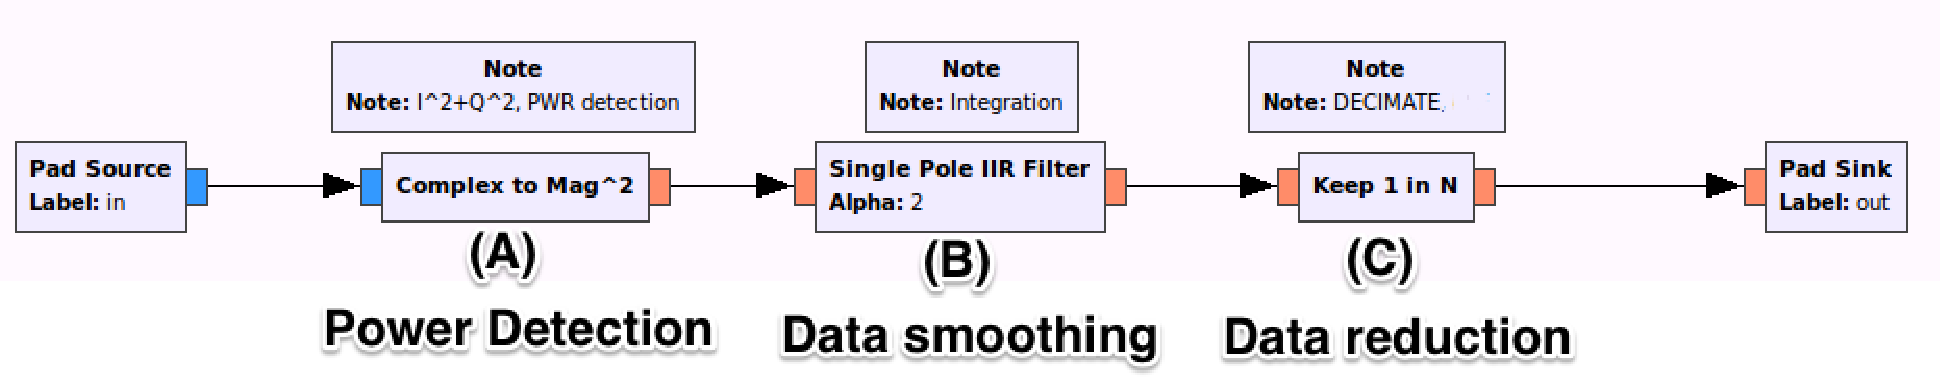
\includegraphics[width=17cm]{Images/TPR_grc.png}
\isucaption{A block diagram of the power detection, low pass filter and decimation block used for total power measurements.}
\label{square_block}
\end{figure}
}

For both a traditional radiometer and a SDR based radiometer the output of this total power information will fluctuate rapidly.  To smooth this signal we will pass this signal through a low pass filter which is shown in Figure \ref{square_block} as block B.  Filtering will be discussed in the next section.

\subsection{Data filtering}

Output from the square-law detector is noisy due to the rapid fluctuations in the signal.  Figure \ref{square_raw} shows an example of this raw output.  This makes detecting small changes in power difficult (i.e. hinders sensitivity).  

{\begin{figure}[h!tb] 
\centering
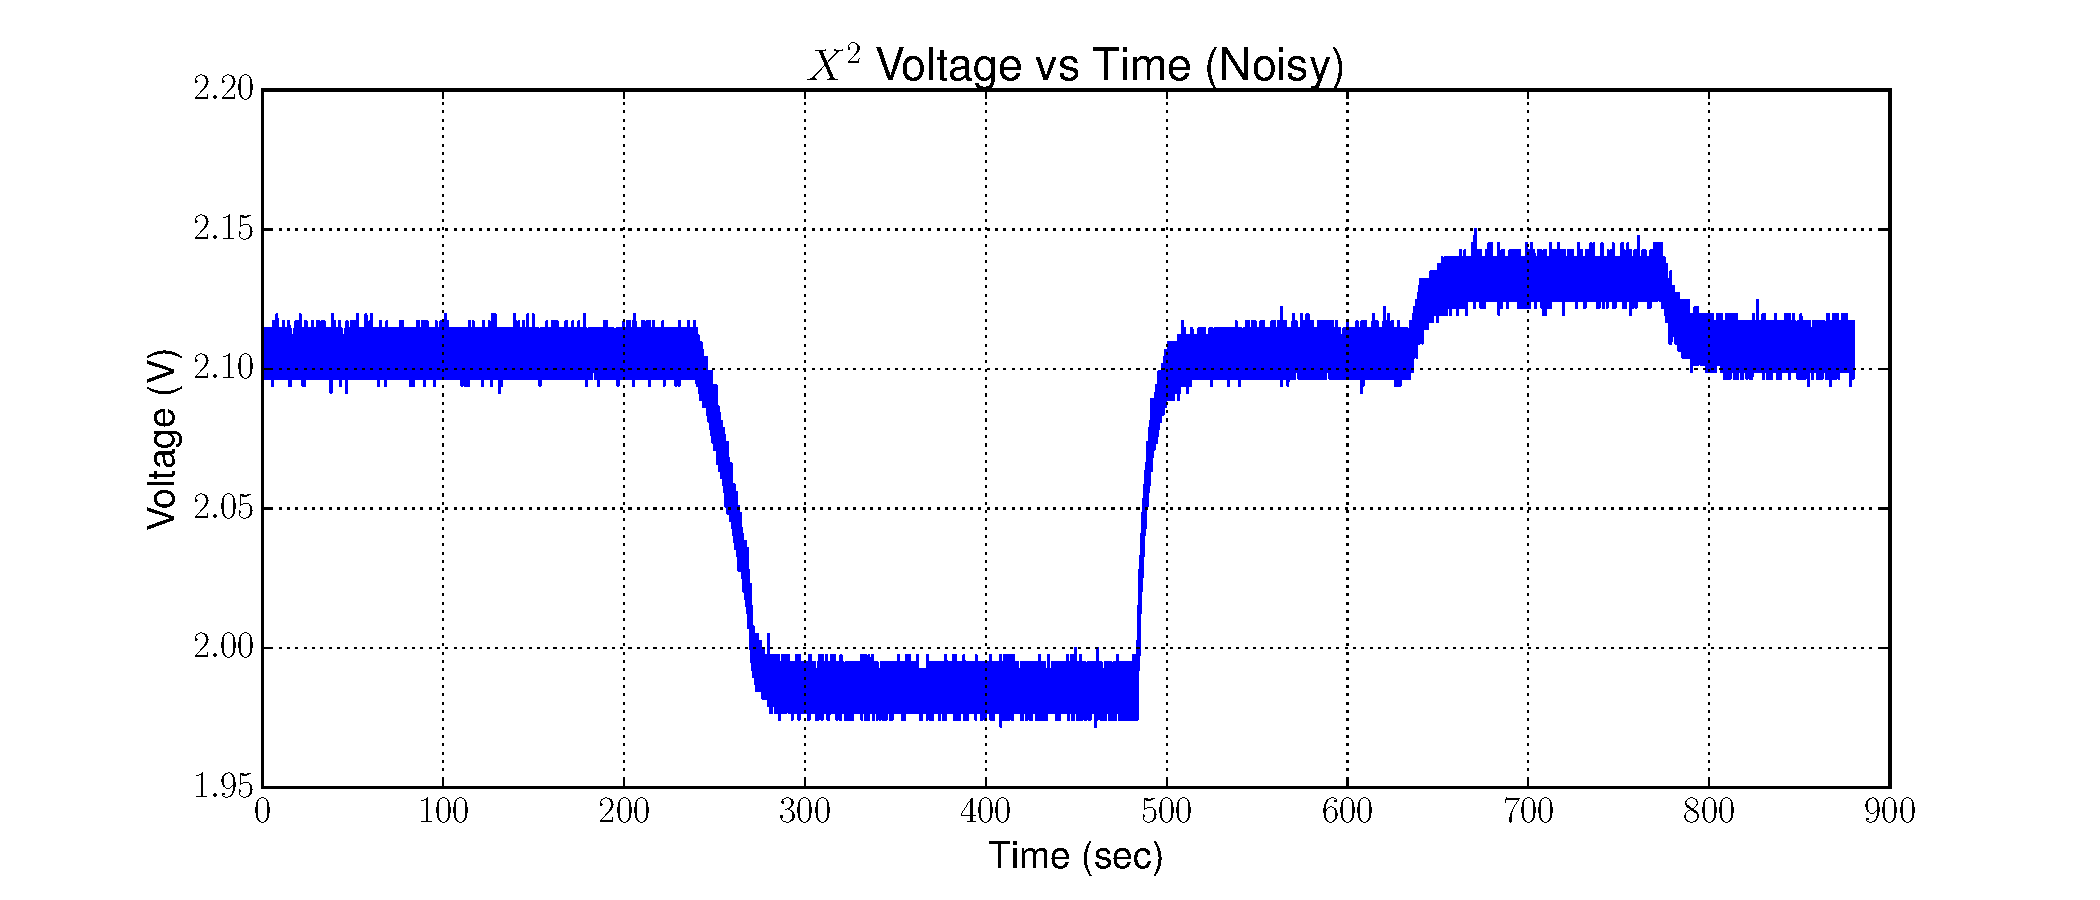
\includegraphics[width=17cm]{Experiments/Exp1/noisy_voltage.pdf}
\isucaption{Power measurements from a square law detector before filtering}
\label{square_raw}
\end{figure}
}

A traditional radiometer will use an integrator, which is equivalent to a low pass filter, to smooth the output from the square-law detector.  This low pass filter is implemented as a simple RC circuit as shown in Figure \ref{rc_circuit}.  

{\begin{figure}[h!tb] 
\centering
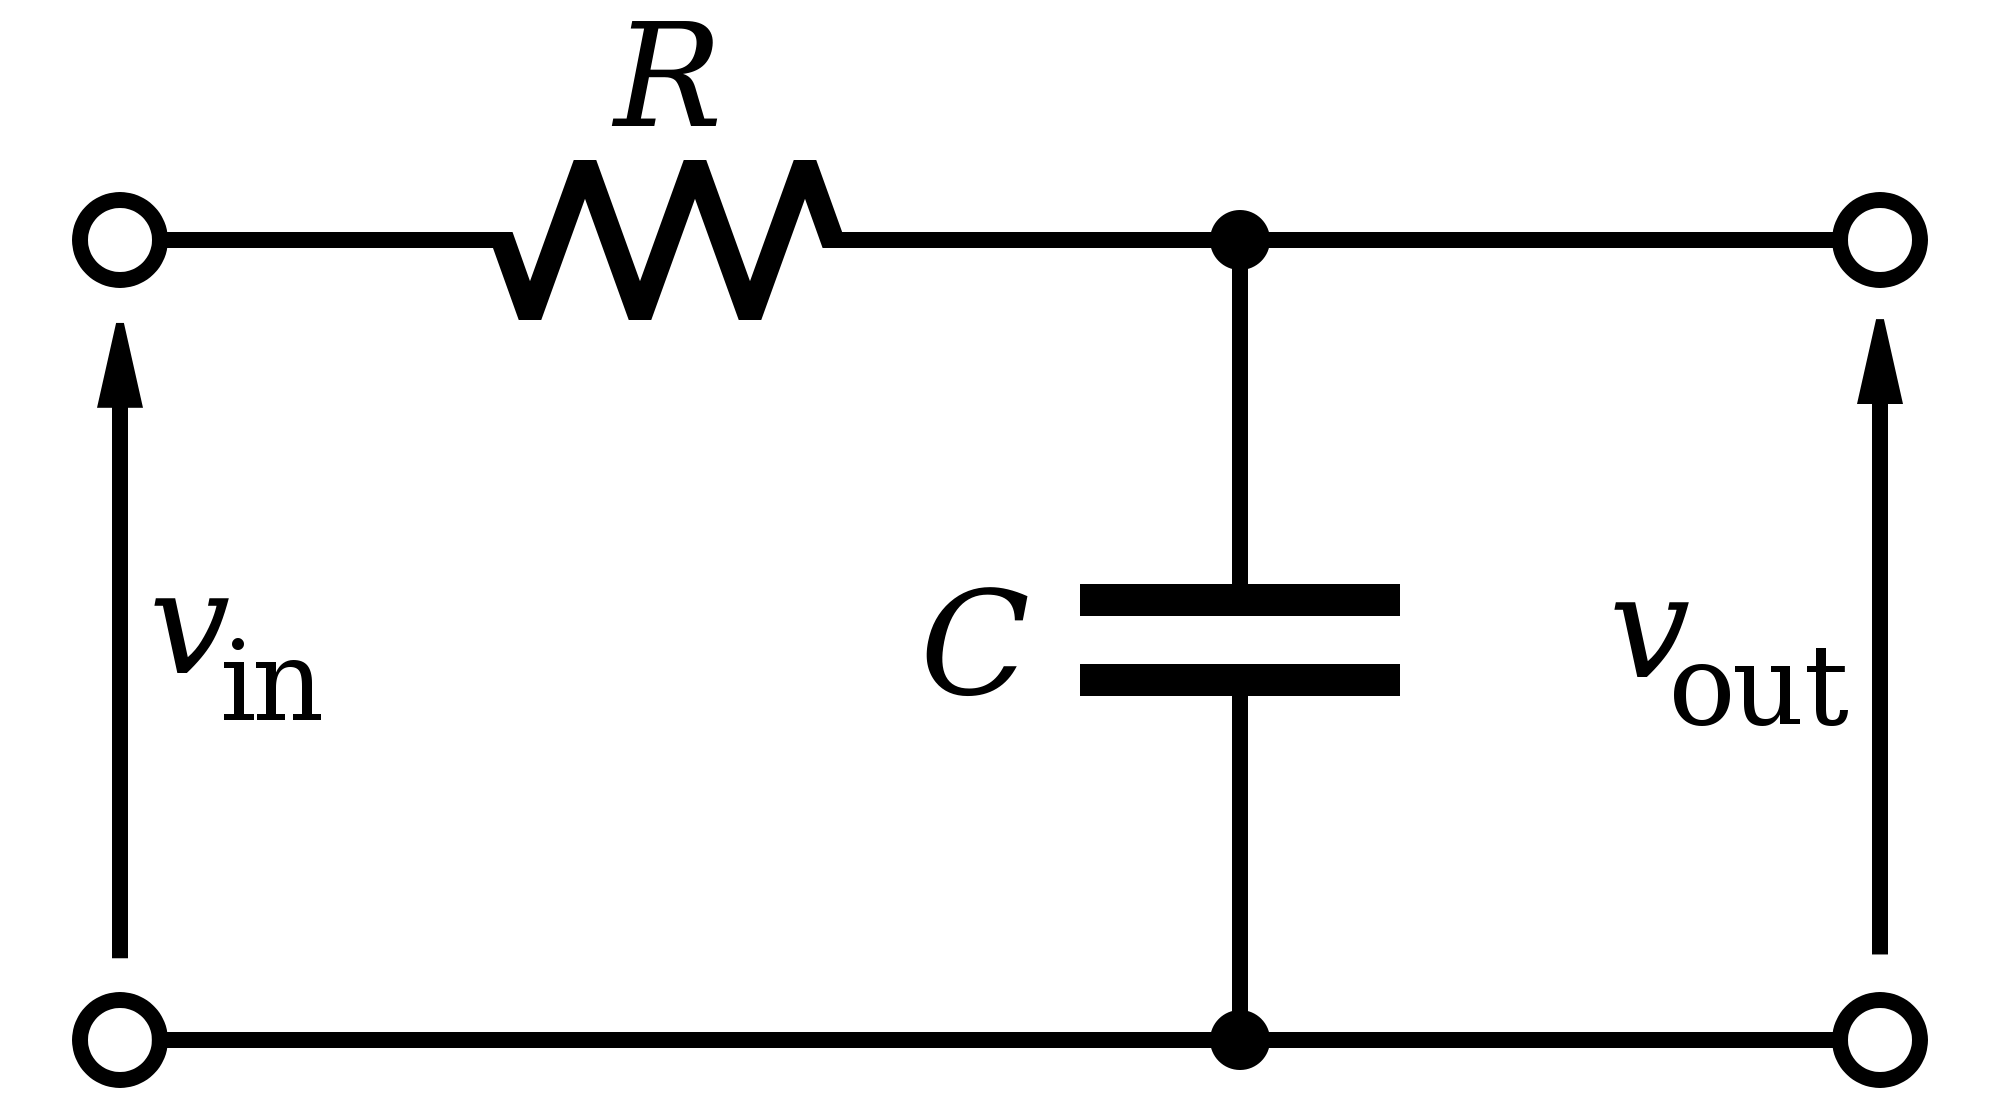
\includegraphics[width=11cm]{Images/rc_lpf.png}
\isucaption{A simple RC circuit.}
\label{rc_circuit}
\end{figure}
}

This low pass filter allows us to reduce the noise and this results in Figure \ref{square_raw_filt}.  

{\begin{figure}[h!tb] 
\centering
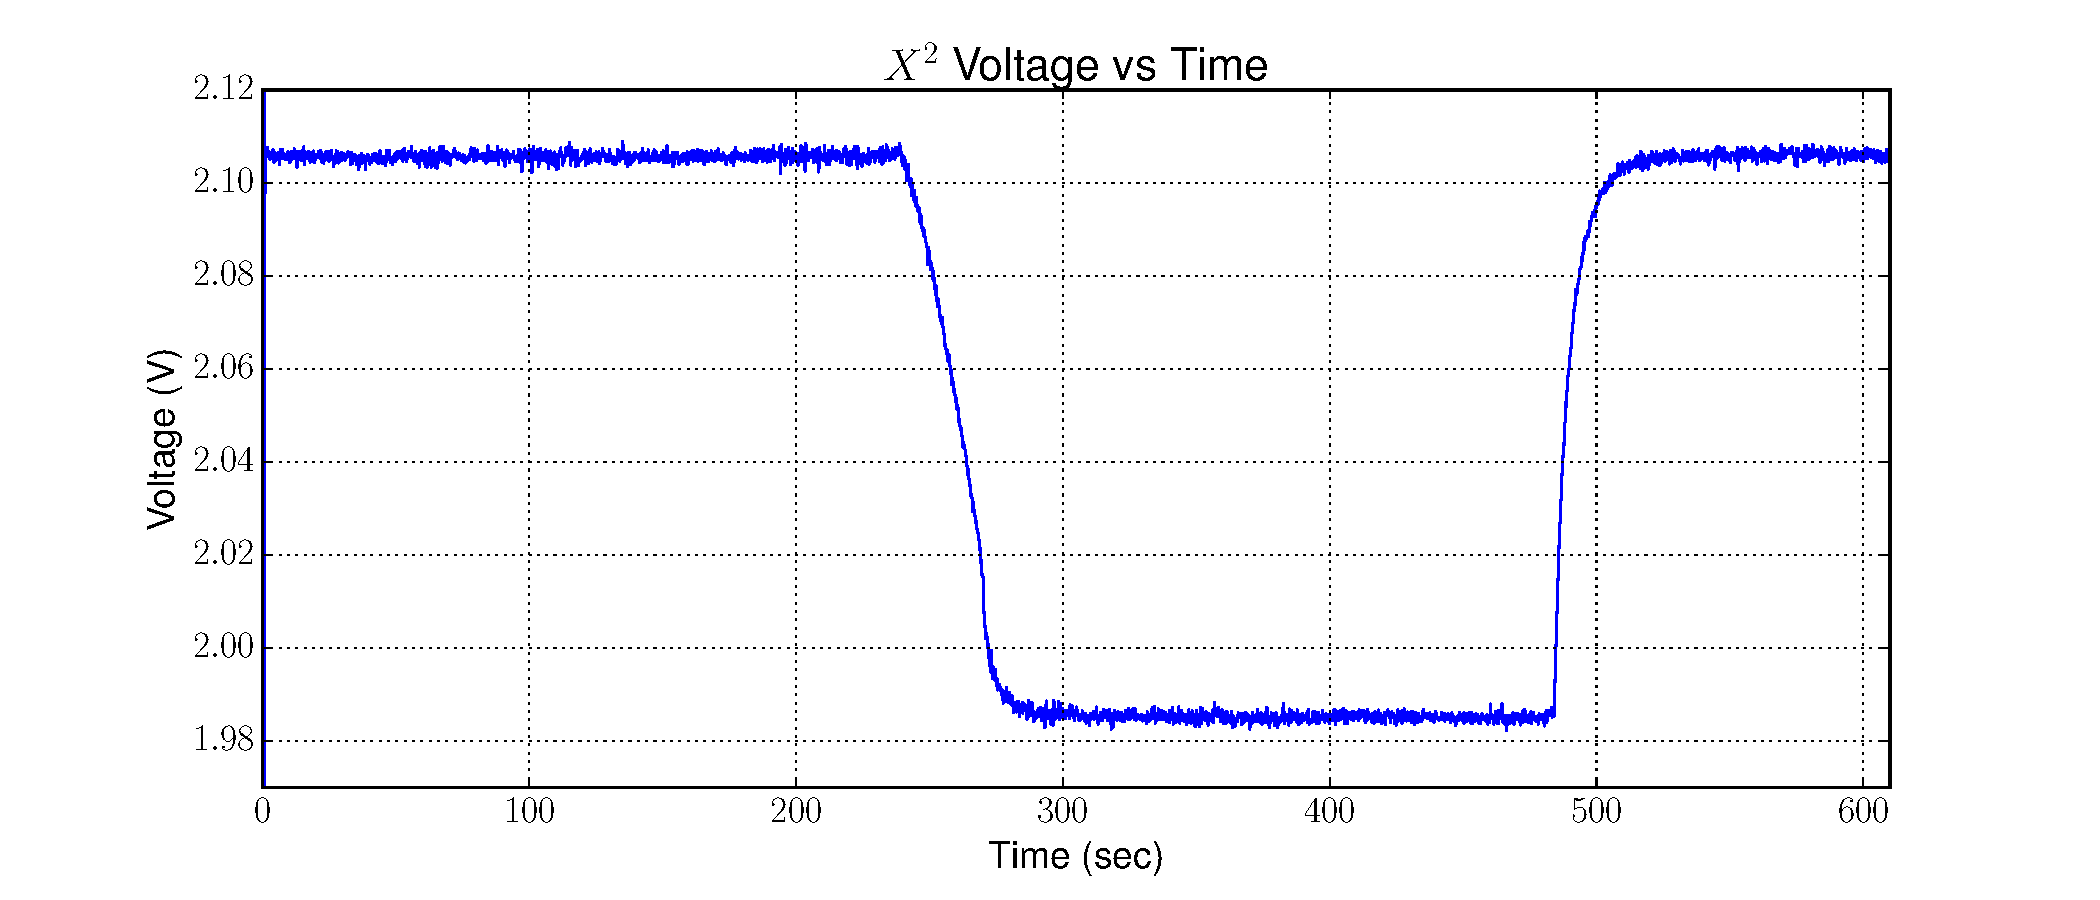
\includegraphics[width=17cm]{Experiments/Exp1/x2_filter.pdf}
\isucaption{Power measurements from a square law detector after filtering}
\label{square_raw_filt}
\end{figure}
}

This RC filter is described by the Laplace transform of its impulse response.  This RC filter is shown in Equation \ref where $K$ is the gain of the filter, $\tau$ is the time constant of the filter and $s$ is the Laplace transform variable.

\begin{equation}\label{RC_laplace}
\frac{Output}{•Input} = K \frac{1}{\tau s + 1}
\end{equation}

We can now look at the impulse response of this filter as shown in Figure \ref{rc_response}.  Figure \ref{rc_response} shows an impulse function used as the input to a RC filter.

{\begin{figure}[h!tb] 
\centering
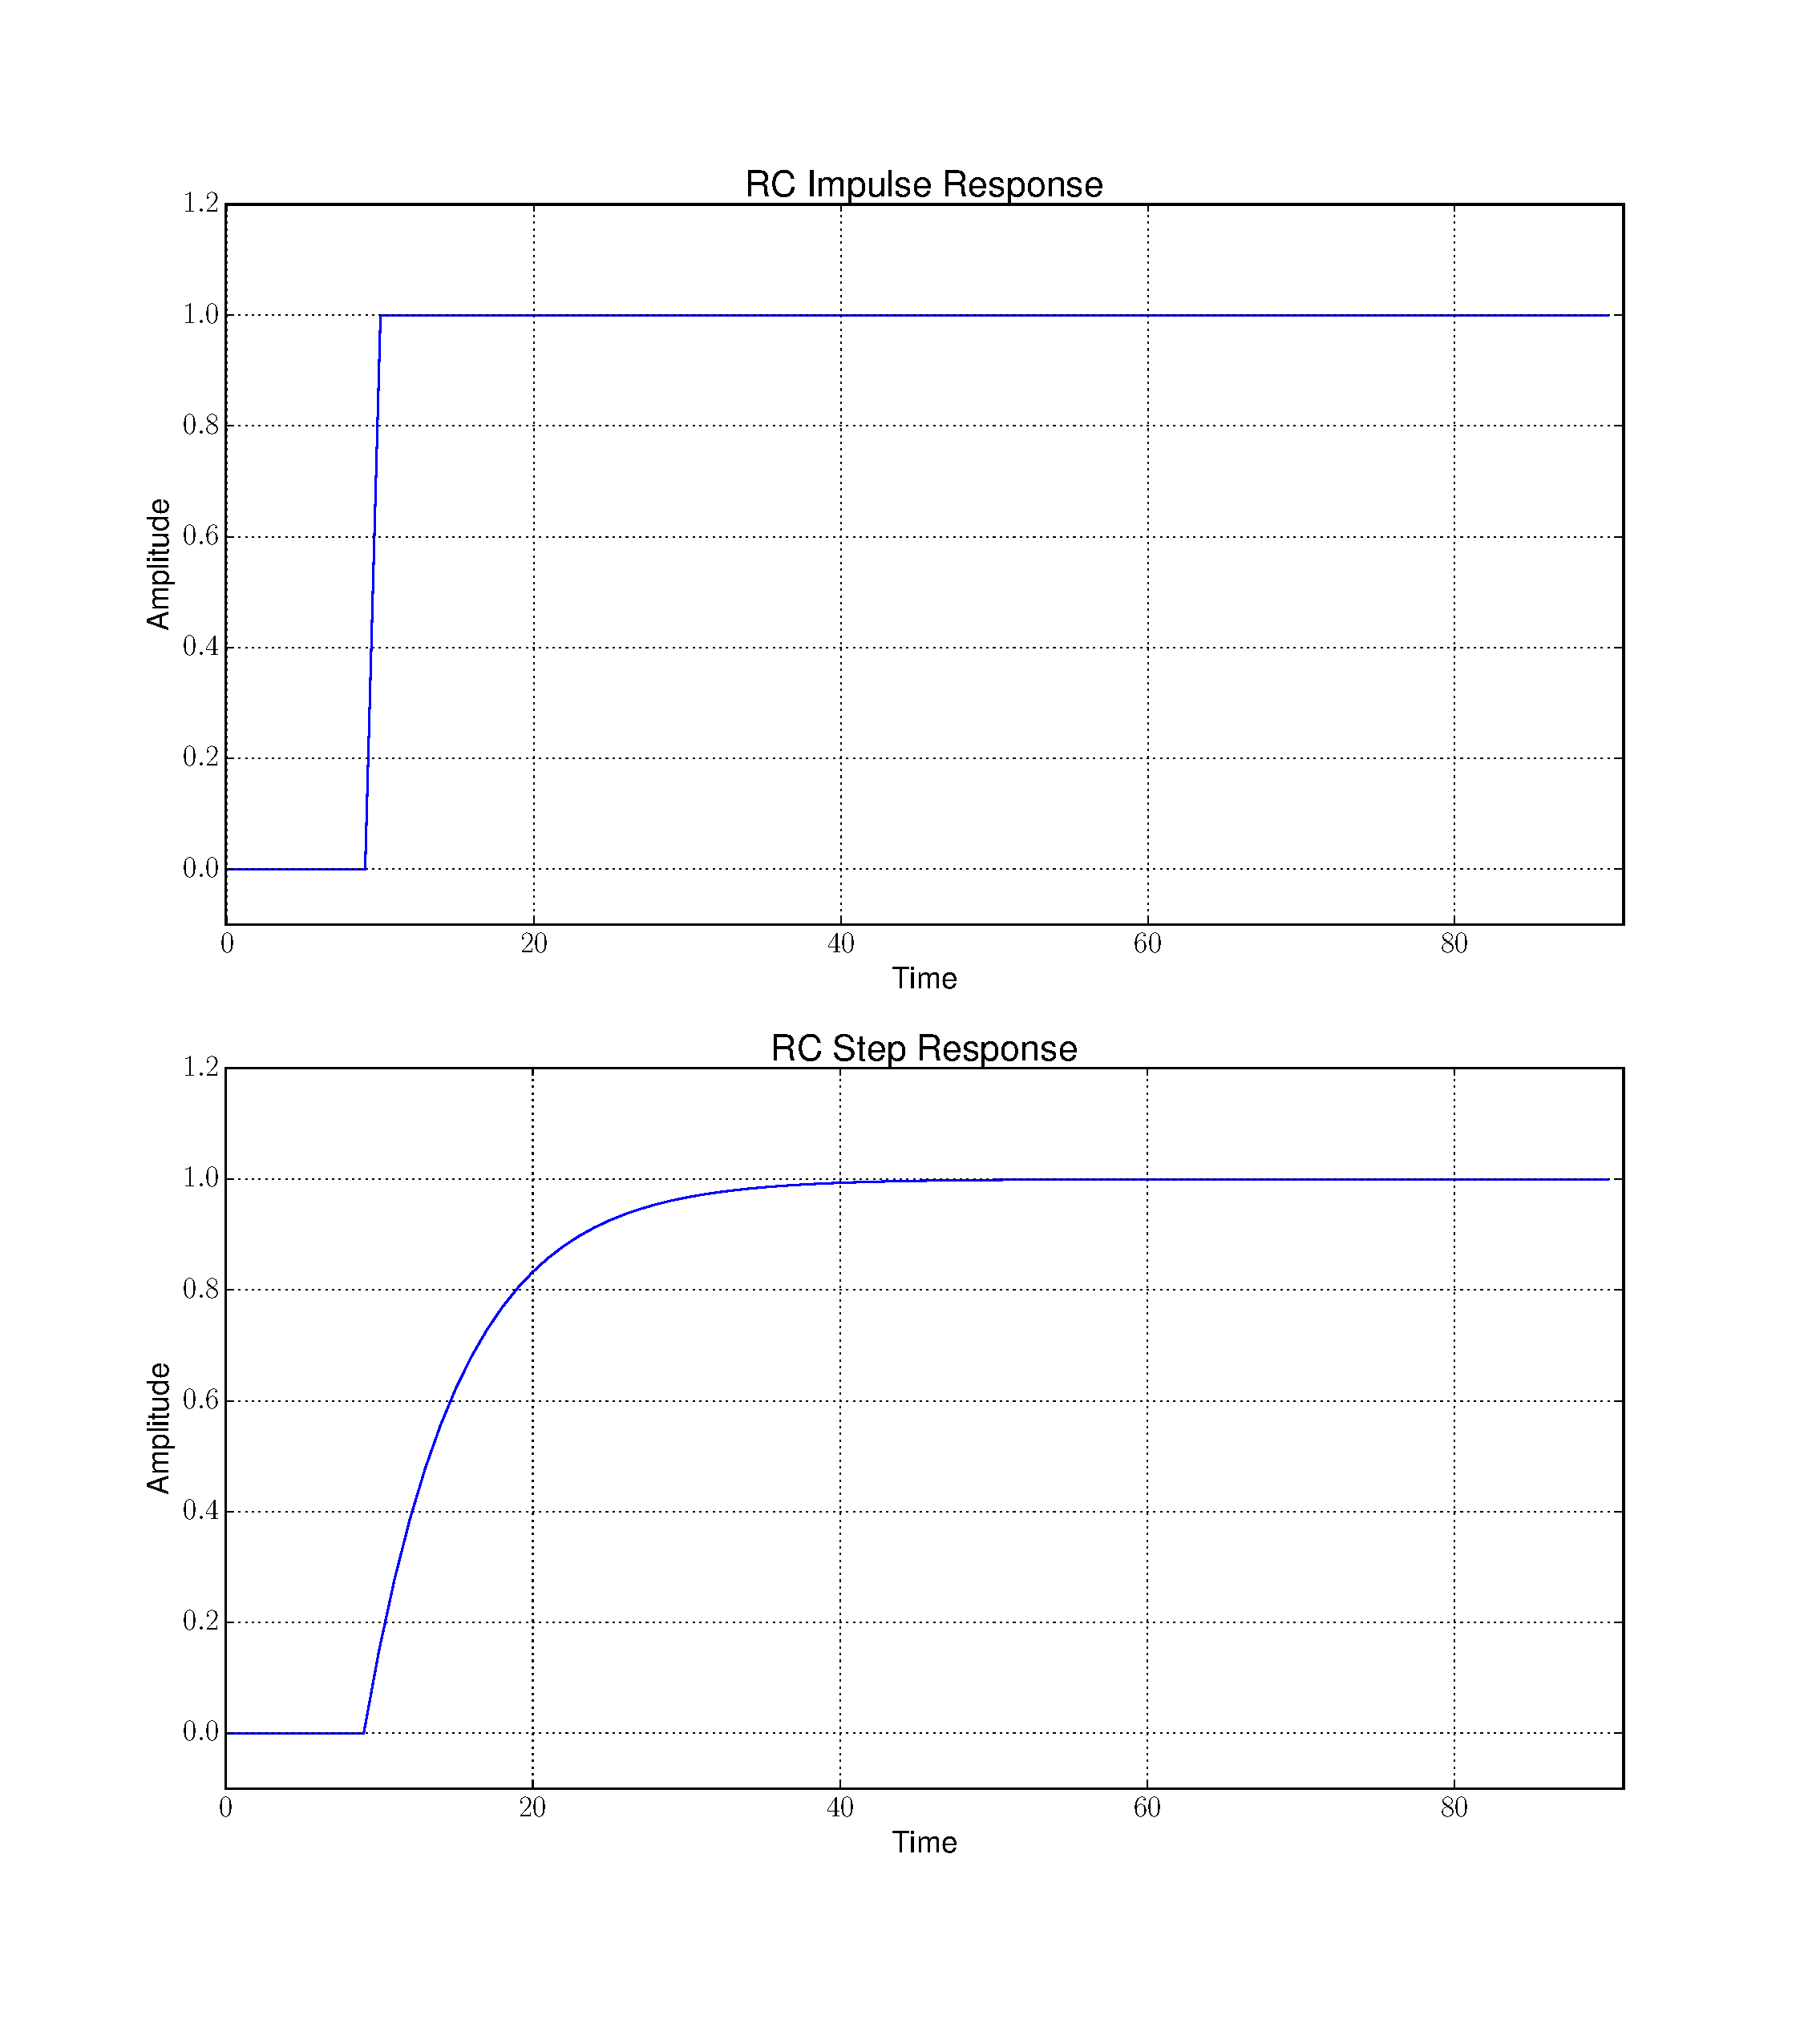
\includegraphics[width=17cm]{Experiments/Exp6/rc_response.pdf}
\isucaption{Impulse input and the response of a RC low pass filter}
\label{rc_response}
\end{figure}
}

%A common solution used by radiometers is to use an integrator, implemented as a RC low pass filter to smooth out this signal.   An integrator averages a signal over time, which effectively reduces the rapid fluctuations in the output.

%A traditional radiometer will use a simple Resistor and Capacitor (RC) circuit to accomplish this.  Because our signal, even a noisy one, has a frequency component, this RC circuit acts like a low pass filter.  Thus the higher frequency "noise" is filtered out.

%To improve our sensitivity, and reduce the rapid fluctuations in the power measurements, we integrate the power measurements.  This gives an average of the signal and reduces the fluctuations in the output.  This helps to improve the sensitivity of the radiometer as seen in equation \ref{NEAT_EQ}.  Chapter \ref{ch:background} section \ref{int_filt} goes in to more detail on how an analog integrator works.  The digital equivalent to a integrator is a Finite Impulse Response (FIR) filter.

To implement this low pass filter as a digital filter, a single pole Infinite Impulse Response (IIR) filter is used.  We can examine how a IIR filter is identical to a RC filter by looking at the impulse response of this filter as we did with the RC filter impulse response.

A single pole IIR filter is also known as a recursive filter as the mathematical expression used to describe this filter is a recursive function shown in Equation \ref{iir_recursive}.  

\begin{equation}\label{iir_recursive}
y[n] = a_0 * x[n] + b_1 * y[n-1]
\end{equation}

In Equation \ref{iir_recursive}, our discrete output ($y[n]$) is defined as the input signal ($x[n]$) and is added to the previous sample calculated.  The coefficients, $a_0$ and $b_1$ then define the impulse response of the filter.

Figure \ref{iir_response} shows the discrete impulse input given to the system and the output response.  This response is calculated using Equation \ref{iir_recursive}.

{\begin{figure}[h!tb] 
\centering
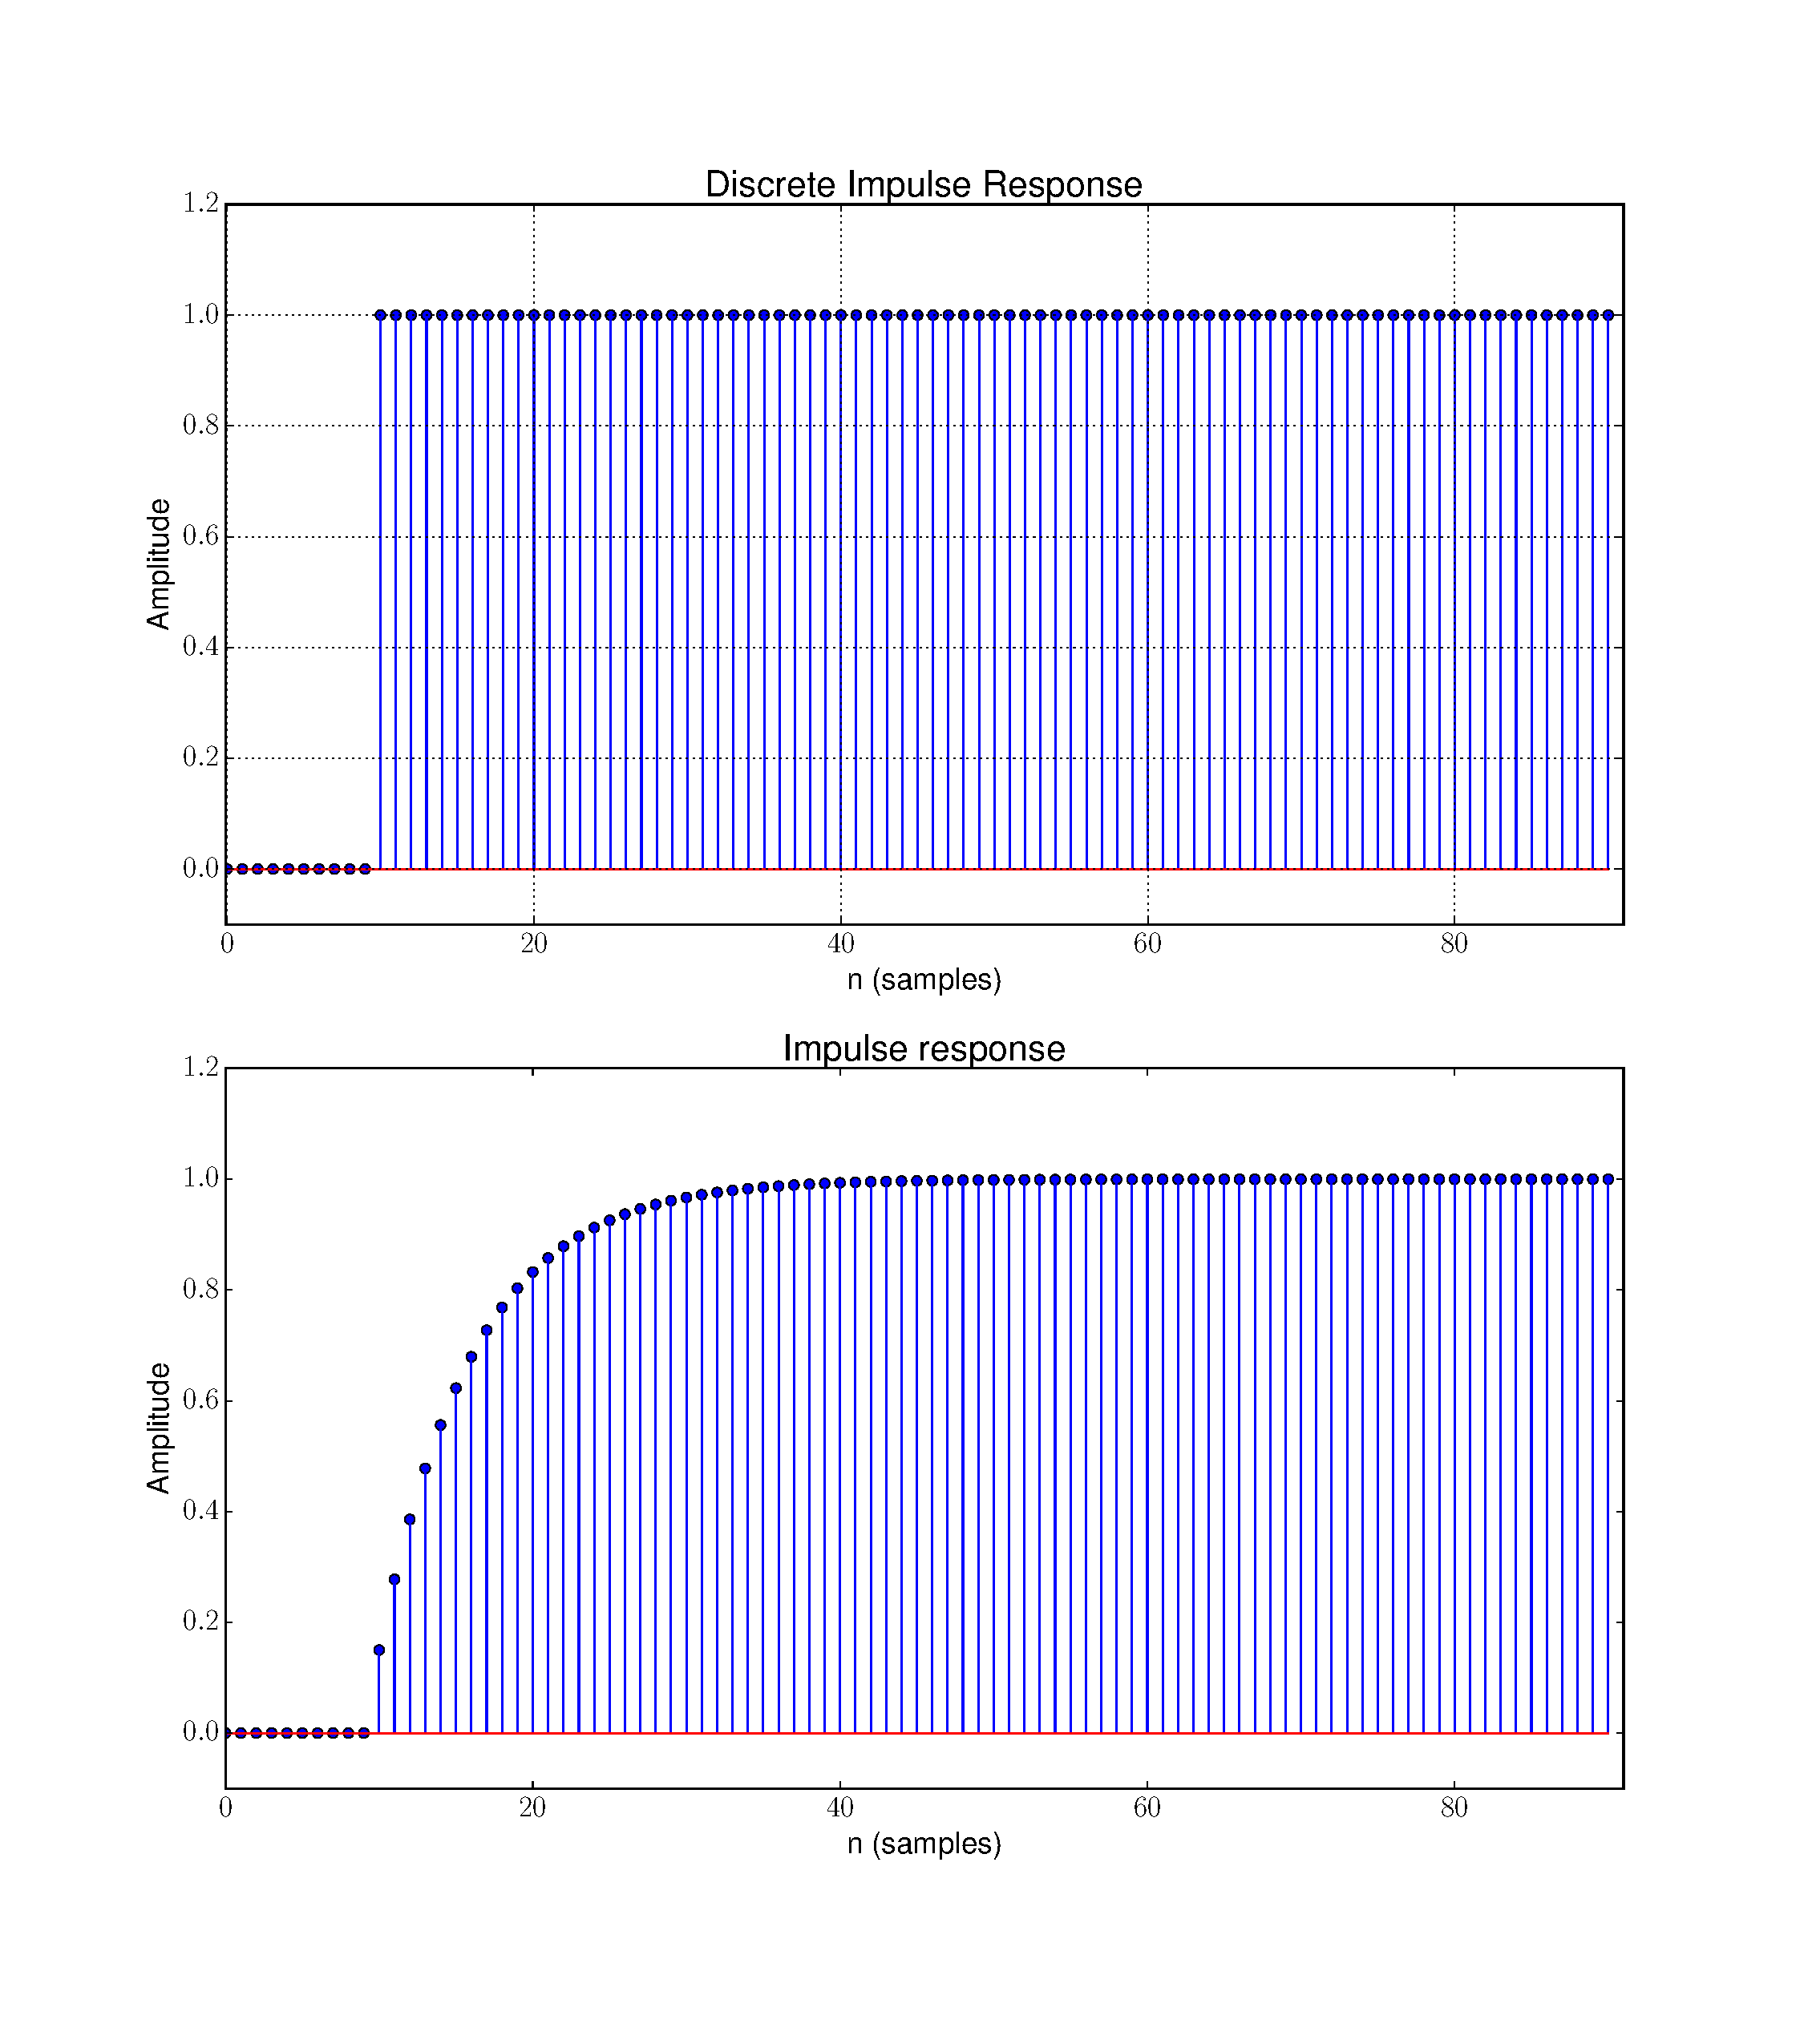
\includegraphics[width=17cm]{Experiments/Exp6/iir_response.pdf}
\isucaption{Impulse input and the response of a RC low pass filter}
\label{iir_response}
\end{figure}
}

It can be seen that Figure \ref{iir_response} is identical to Figure \ref{rc_response} except that it is using discrete values.  Therefore are single pole IIR filter functions identically to a RC low pass filter.  

%\begin{equation}\label{IIR_Transfer}
%H(f)=\frac{\displaystyle\sum\limits_{i=0}^{P} b_i z^{-i}}{1+\displaystyle\sum\limits_{j=0}^{Q} a_j z^{-j}}
%\end{equation}

%To implement this as a digital filter, a Finite Impulse Response (FIR) or Infinite Impulse Response (IIR) can be used.  A FIR filter, also known as a non-recursive filter, is a digital filter that can take an impulse signal and decays to zero after a finite number of iterations.  Equation \ref{FIR_Eq} shows the output of this filter ($y_N$) with the input $x_n$, where $P$ defines the order of the filter and is a weighted average of the most recent $P$ inputs.  The array $c_i$ holds $P$ arbitrary constants.  These values define the frequency response of the FIR filter.  

%\begin{equation}\label{FIR_Eq}
%y_n=\displaystyle\sum\limits_{i=o}^{P} c_ix_{n-i}
%\end{equation} 

%An Infinite Impulse Response (IIR) filter, also known as a recursive filter, is the same as the FIR filter, except a summation term is added which feeds back the previous output.  Equation \ref{IIR_eq} shows that a FIR filter is a IIR filter, with an extra summation term added[\cite{Cross}]. This term has the $d_j$ array which holds the weighting coefficients for feeding back the previous $y_{n-j}$ outputs.  IIR filters can produce better results with less computational cost.  However, they are harder to design and may become unstable if not designed properly.

%\begin{equation}\label{IIR_eq}
%y_n=\displaystyle\sum\limits_{i=o}^{P} c_ix_{n-i}+\displaystyle\sum\limits_{j=1}^{Q} d_jy_{n-j}
%\end{equation}

%To design either a FIR or IIR filter, the coefficient arrays $c_i$ and $d_j$ are often referred to as "taps".  These tap values define the filter as shown in Equation \ref{FIR_Eq} and Equation \ref{IIR_eq}.  To generate these tap values, GNURadio provides a filter design program.  This program is both a standalone GUI program and can also be called from within a GNURadio Companion.  The sampling rate, frequency response and cutoff frequency can be sent to the program to calculate the required taps.  

%In terms of computational and memory requirements, the more taps we generate the more accurate the filter will become.  It will also be possible to design a filter with a faster (steeper) frequency response with more taps.  However, each tap requires memory for it to be stored and also requires computation against the input signal.  Therefore more taps also require more computational and memory requirements.  

%Both filters produce the same result by giving the average of the input signal.  An IIR filter however often uses less computational power than a FIR filter.  Because of this, an IIR filter was used in defining our integrator in a software defined radio based radiometer.

%To get a better understanding on how the digital IIR filter relates to the RC filter analog, we need to look at the frequency response of the digital filter.  We can do that by looking at the Fourier Transform and the relationship of the input to the output in the frequency domain in Equation \ref{Fourier_IIR} where $f$ is our frequency in Hz and $T$ is our time between samples in seconds.  

%\begin{equation}\label{Fourier_IIR}
%H(f)=\frac{\displaystyle\sum\limits_{i=0}^{P} b_i z^{-i}}{1+\displaystyle\sum\limits_{j=0}^{Q} a_j z^{-j}}
%\end{equation}

%Our IIR filter needs to behave like a low pass filter to filter out the high frequency components.  As discussed earlier, an analog radiometer might do this with a simple RC circuit.  Figure \ref{rc_circuit} shows what this circuit looks like.

%In Figure \ref{rc_circuit}, the input is $V_{in}$, the resistance value is $R$, the capacitance value is $C$ and the output is $V_{out}$.  This circuit can be represented by Equation \ref{eq:rc_circuit_eq}.

%\begin{equation}\label{eq:rc_circuit_eq}
%\frac{V_{in}-V_{out}}{R}=C\frac{dV_{out}}{dt}
%\end{equation}

%Equation \ref{eq:rc_circuit_eq} represents the differential equation relating the input voltage $V_{in}$ to the output voltage $V_{out}$.  We can substitute the input to the RC circuit ($V_{in}$) as the input to Equation \ref{IIR_eq} or $x_n$.  The output of our RC circuit ($V{out}$) can also be expressed as the output in Equation \ref{IIR_eq} which is $y_n$.  However, in order to do that we must move from the continuous domain to the discrete domain that our digital filter operates in.  This is done by showing the relationship between our sampling frequency $f_s$ and our period or time between samples, $T$ and is shown in Equation \ref{sampling_rate_eq}.

%\begin{equation}\label{sampling_rate_eq}
%T=time between samples=\frac{1}{f_s}
%\end{equation}

%We can now relate our input voltage ($V_{in}$) to the input to our IIR filter ($x_n$) by multiplying our voltage input to th our period and the number of samples, $n$. shown in Equation \ref{input_IIR} and the output voltage shown in Equation \ref{output_IIR}.

%\begin{equation}\label{input_IIR}
%x_n=V_{in}(nT)
%\end{equation}

%\begin{equation}\label{output_IIR}
%y_n=V_{out}(nT)
%\end{equation}

%Next we rewrite our difference equation by substituting $x_n$ and $y_n$ into Equation \ref{eq:rc_circuit_eq} which results in an approximated finite difference equation shown in Equation \ref{diff_xn_yn}.

%\begin{equation}\label{diff_xn_yn}
%\frac{x_n-y_n}{R}=C\frac{y_n-y_{n-1}}{T}
%\end{equation}

%We can now solve for $y_n$ algebraically and this results in our final Equation \ref{final_IIR_RC}.

%\begin{equation}\label{final_IIR_RC}
%y_n=\frac{T}{T+RC}x_n+\frac{RC}{T+RC}y_{n-1}
%\end{equation}

%Equation \ref{final_IIR_RC} shows an IIR filter that has a frequency response that closely approximates an RC circuit.  The approximation improves as $T$ approaches zero or our sampling rate approaches infinity.

%To design the filter we need to look at what our desired cut-off frequency needs to be.  For a RC filter, our resistance and capacitance define our cutoff frequency ($f_c$) and has the relationship shown in Equation \ref{fc_RC}.

%\begin{equation}\label{fc_RC}
%f_c=\frac{\sqrt{3}}{2\pi RC}
%\end{equation}

%Given our desired cutoff frequency we can determine our combined $RC$ value by rearranging Equation \ref{fc_RC} algebraically to Equation \ref{RC_fc}.

%\begin{equation}\label{RC_fc}
%RC=\frac{\sqrt{3}}{2\pi f_c}
%\end{equation}

%The $RC$ values are also referred to as the time constant of the circuit and we do not need to find the individual R and C values.  An example of how we can find the coefficients of our IIR filter, given a desired cutoff frequency of $f_c$ is shown next.  

%For a low pass filter, we want a cutoff frequency ($f_c$) of 1000 Hz.  Given this and using Equation \ref{RC_fc} we can determine our time constant to be 2.757 x $10^-4$ or 275.7 microseconds.  If our sample rate is 1 MHz, then our $T$ value is 1 x $10^-6$ or 1 microsecond.  Plugging these values into Equation \ref{final_IIR_RC} results in the coefficient $c_0 = 0.0036$ and $d_1=0.9964$.  

GNURadio includes a program that allows us to define our filter and it will generate the coefficients and taps needed for our filters.  Chapter \ref{ch:results} goes into more depth on this program.

%The $RC$ term gives us our time constant of the circuit and can be used to calculate out our coefficients.  We are not concerned about the actual values of R and C with our IIR filter, instead we just need the product of R and C.  


\subsection{Bandwidth limitation}
A traditional radiometer will use filters to define the bandwidth of the radiometer.  A software defined radio based radiometer however uses the sampling rate to define the bandwidth.  This sample rate may be adjusted but will be limited by the computational power available.  The higher the sample rate, and therefore the more bandwidth observed, the more computational power needed.  

Additional filtering can be created and used in a software defined radiometer.  These filters are often created using either IIR or FIR filters.  The most efficient method is to restrict bandwidth by setting the sampling rate.  However, these filters can be used to filter out either a narrow band of frequencies or to temporarily reduce the overall bandwidth.  A common application of these additional filters is to remove an offending signal detected by the software defined radio based radiometer.  This method of mitigating signal interference will be discussed in chapter \ref{ch:results}.

\section{Software Defined Radio Based Radiometer Control System}

Like a traditional radiometer, the SDR uses an antenna to look at the target of interest.  SDRs still use an amplification to improve the sensitivity of the SDR. After that stage though, a software defined radiometer is different.  A SDR will sample and generate I and Q values that represents the signal.  From there, this data is sent to a computer to be processed.  We can then use this information to calculate the total power of the signal.  In addition, we can manipulate the signal in other ways such as applying a filter to filter out an unwanted source.

A traditional radiometer will be designed with bandwidth and integration time fixed.  While changes can be made, it requires changes to the radiometers physical hardware.  A Software Defined Radio (SDR) based radiometer however can have both the  bandwidth and the integration time changed.  These changes can even be made while the radiometer is operating since both operations happen in the digital domain.  

Because these values have an impact on the performance of a SDR based radiometer, it is important to have access 


%As we have shown the two of the major components of a traditional radiometer, the power detection and integration of the signal can be replicated in software and therefore can be implemented in a software defined radio.  The information can now be stored, displayed or both for further analysis.  

%There is one component of the software defined radio that we are not able to implement in software and that is with the signal amplification.  This however does play a major role in the performance of the radiometer and is a key element that should not be overlooked.  While this is not implemented in software, it still plays a critical role in our software defined radio radiometer. 

Next we will now look at how we control the software defined radiometer using the software detailed in chapter \ref{ch:background}, section \ref{software_platform} in defining the radiometer.  We will also look at how the data is displayed and stored in the software defined radiometer.

\subsection{Control of the SDR based radiometer through GNURadio}
%The N200 sends all data across the 1 Gbps Ethernet connection to be read in by a host computer running GNURadio.  This data is the raw I/Q values that is read by the on board A/D and processed by the on board FPGA.  An example of a very simple GNURadio software implementation would simply take this data and store the data to a hard drive in a file.  This can be very handy if we want to simply record the data and then process it later.  However, depending on the sample rate, this can consume a large amount of storage.  A short recording can  consume 1-2 GB with a sample rate of 10 Msps.  This simple system also does not give us any immediate feedback on the radiometer and it does not give us controls of the radiometer such as frequency, integration time or other key variables.  Fortunately GNURadio has tools that allows us to build up a very rich application that is able to give us the data we need and control the software defined radio as well.

%The GNURadio Companion software allows us to create python code that is used to not only receive the data from the SDR but also perform signal processing on the incoming information.  Additional controls are added that allow for tuning of the signal processing parameters and control of the radio functions.  With this we can build up an application that can be run on any computer that is capable of running GNURadio. 

A GUI is designed to allow control of several key functions of the SDR based radiometer.  This GUI is shown in Figure \ref{radiometer_gui}. 

{\begin{figure}[h!tb] 
\centering
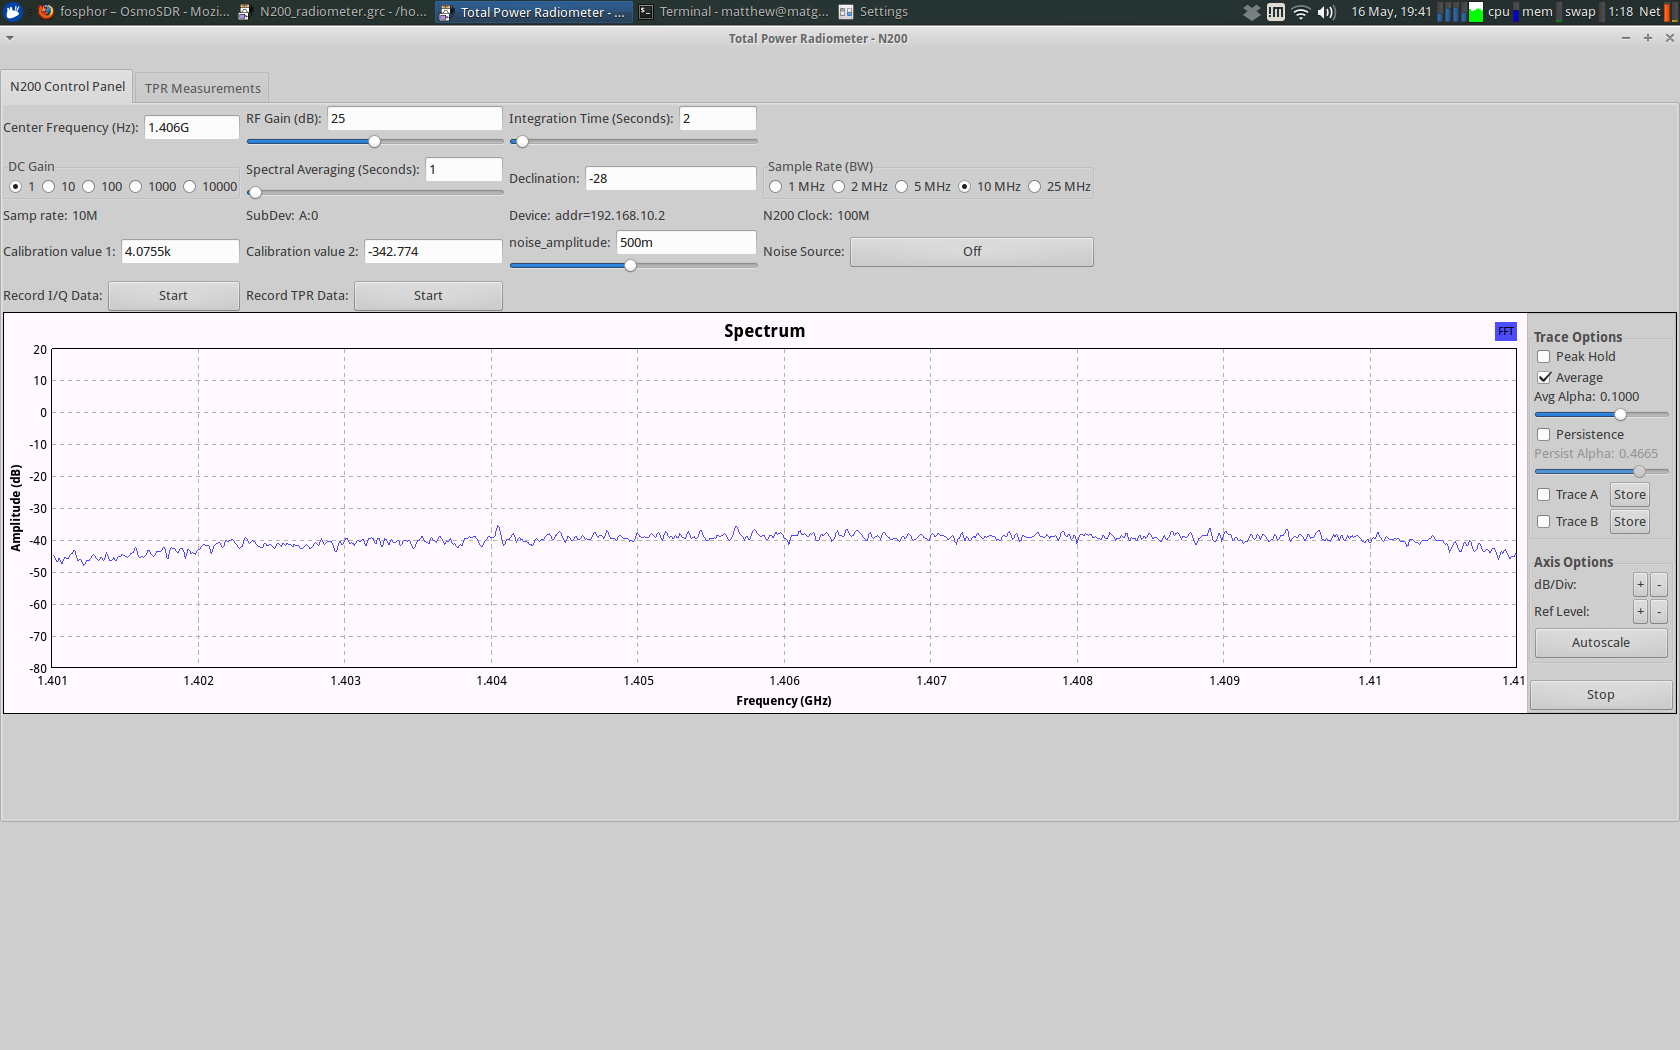
\includegraphics[width=17cm]{Images/radiometer_gui.png}
\isucaption{A screenshot of the interface made for communication with and controlling the software defined radio}
\label{radiometer_gui}
\end{figure}
}

This interface is able to control several key aspects of the radio hardware within the SDR.  This has the impact of affecting the behavior of this software defined radiometer as well.  Through this we can control: frequency, sample rate (Bandwidth), integration time, and the gain on the DBSRX2 daughter board.  We will no look at how these controls impact the performance of the radiometer.  

\subsection{Impact of the Controls Related to Radiometry}

Having the ability to control these key aspects of the software defined radiometer allows us to affect the performance of the radiometer.  The $NE\Delta T$, equation \ref{NEAT_EQ}, discussed in chapter \ref{ch:background} outlines what some of these changes affect in a radiometer.

%For any radiometer noise temperature is a large consideration and is critical to the design of the radiometer.  One method to determine how well a radiometer is to look at the sensitivity of the radiometer.  We can do this by looking at the smallest change in temperature the radiometer can see.  We will call this the Noise Equivalent $\Delta T$ or $NE\Delta T$ of the radiometer and is equation \ref{NEAT_EQ} covered in chapter \ref{ch:background}.

$\beta$ can be changed by changing the sample rate of the SDR.  The sample rate effectively controls the bandwidth in which the SDR is operating at.  This also gives us a band-pass filter as well, since the SDR will not respond to frequencies outside of this bandwidth.  

$\tau$ is the integration time for the radiometer.  This parameter is set by the user through the GUI and allows us to change the integration time in seconds.

We will now look at how this data is displayed by the SDR based radiometer.

%\subsection{GNURadio Data Handling}
%Once we have the data that has been processed by the software defined radio we will want to display this information and be able to store the data so we can analyze it later if needed.  Data display is handled by GNURadio by plotting the total power over time.  This allows the user to be able to visualize the total power and be able to determine if the total power has increased or decreased over the time window shown.  

%We also have the ability to look at a signal in terms of frequency versus amplitude.  This allows looking for any unusual signals that may be interfering with the system or causing erroneous data with our radiometer.  The data stored from this program is covered in more detail in chapter \ref{ch:results}.  

%Finally, we will want to store the data so we can do additional analyses on it at a later time.  The GNURadio program allows us to store the data in two formats.  The first format is storing the raw I/Q data from the radiometer.  This format allows us to playback the data through GNURadio at a later time.  This can be useful for if we wish to change parameters in GNURadio such as bandwidth or integration time.  It is also a good diagnostic tool as we can check that the signal coming in is clean or if we need to apply additional filters to remove an unwanted signal.

%The second format is the total power that has been calculated by the radiometer.  This file is much smaller since much of the signal information has now been reduced to simple power versus time information.  This allows for easy manipulation through any math program such as Matlab for analysis.  

\subsection{GNURadio Data Display}
The information from the software defined radio can be displayed through GNURadio to show a number of things.  Since we have both frequency and magnitude information we can display this information.  We are able to also display the information that shows the total power that is being seen by the radiometer as well.

{\begin{figure}[h!tb] 
\centering
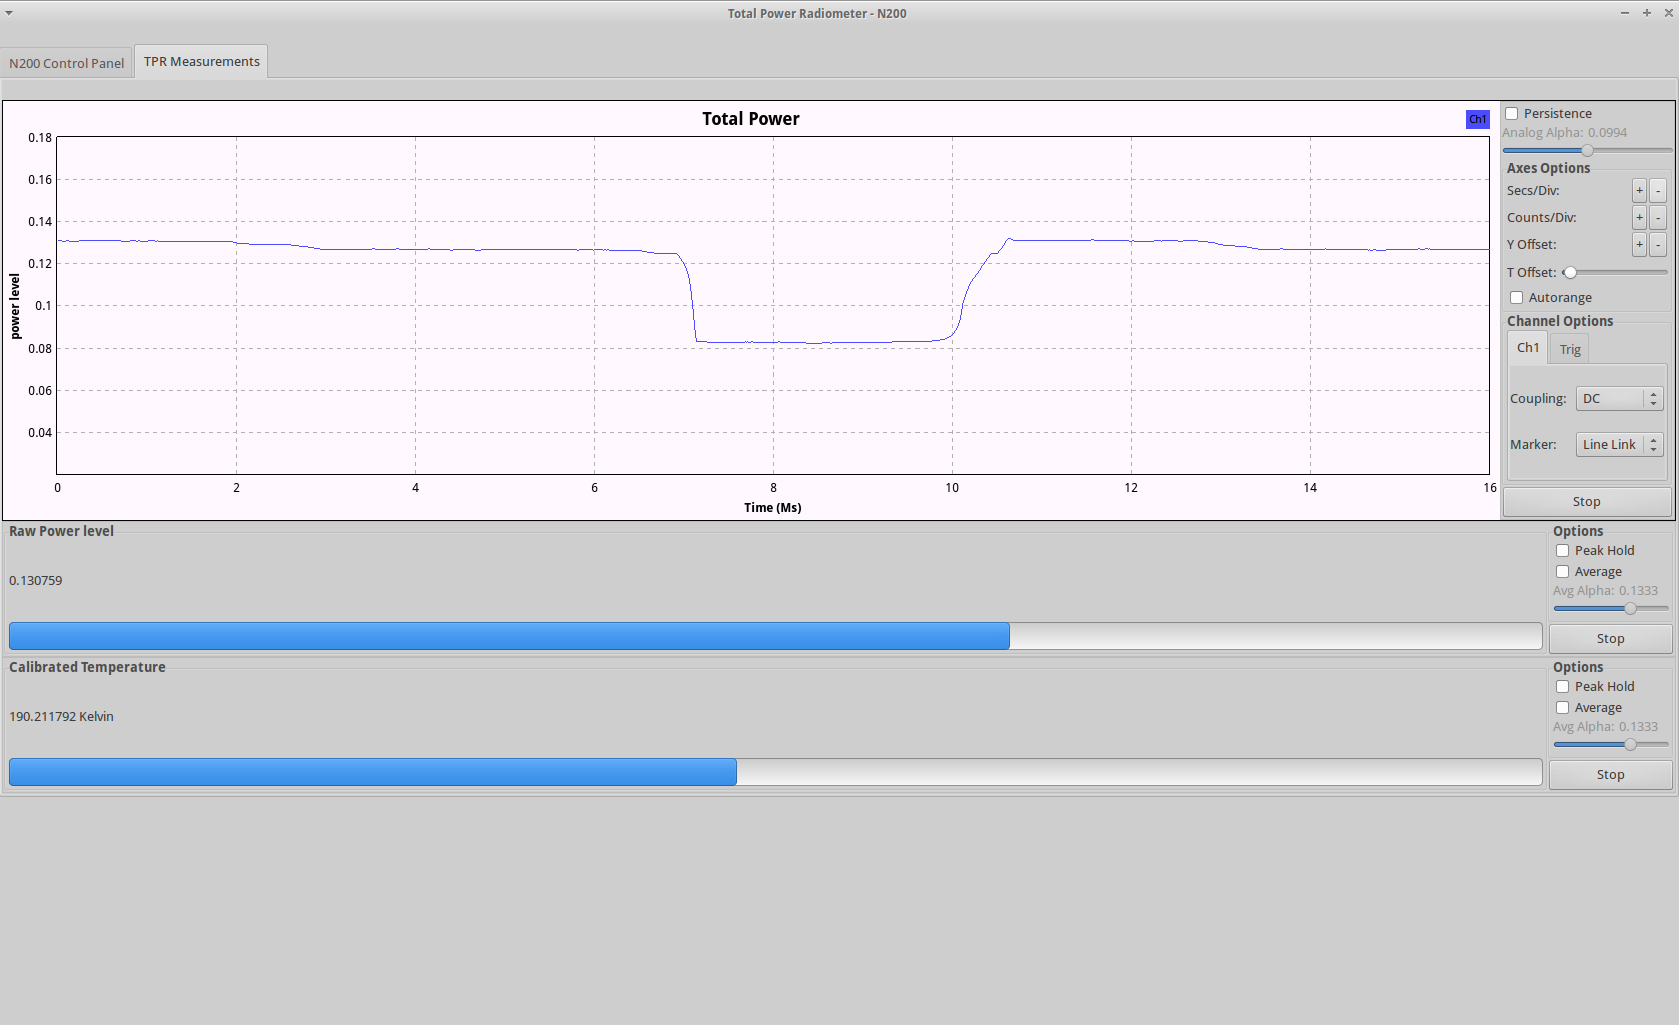
\includegraphics[width=17cm]{Images/Lab1_TPR_at_end_exp.png}
\isucaption{A screenshot showing the ticker tape display for the total power readings.  In addition, raw and calibrated noise temperature is shown below.}
\label{radiometer_tpr_display}
\end{figure}
}

We are not limited to just total power from the radiometer.  If the radiometer has been calibrated, those calibration points can be entered and GNURadio can calculate the calibrated noise temperature.  

%Additional information may also be added as needed.  For example, we are able to view the full spectrum that the radiometer sees.  This can be a useful tool for looking at potential RFI issues.  
%----------------------------------------------------------------------------------
%Everything below this needs to be moved/shifted or deleted

%\section{Square-law Detector Performance}
%The Square-law detector was added to our system in order to give us another reference point and to help verify the power output that the software defined radio.  Performance of our square-law detector is based on two items; the sensitivity of the diode used in the square-law detector and the analog to digital converter used to convert the analog voltage to a digital value.  The sensitivity of this device accounts for most of the performance factor of the system.  In our system the output of this square-law detector is then feed directly into an analog to digital converter.  Therefore, the performance of this A/D converter needs to be accounted for as well [\cite{Terlep}].  

%For our square-law detector, it has a noise output of $25nV/ \sqrt{Hz}$ at 100 kHz and will detect a signal as low as $-60$ dBm.  This works will with our needs since the RF front end brings the noise floor to approximately $-30$ dBm.
